% RETIRED 2026-09-09: this August-10 narrative was SUPERSEDED on 2026-09-03 by the co-author
% briefing `HAFiscal_update_for_coauthors.md` (the document of record; its pages are generated
% from that markdown) together with the generated `UPDATES.md` and the annotated build
% (`make pdf-annotated`). Its PDF was removed from the repo (it carried 08-10 numbers); the
% source stays for the record and still builds (`pdflatex HAFiscal_update.tex`). The figure
% panels under HAFiscal_update_figs/ are still rendered by Code/HA-Models/update_figs.py.
% HAFiscal_update.tex — standalone update document (owner ruling 2026-08-10):
% the published artifact (HAFiscal-QE / the locked tables and figures) is
% FROZEN as the reference; this document describes how results under the
% corrected computational machinery differ from those reported there, and why.
% Build: pdflatex HAFiscal_update.tex (twice). Not part of the locked set.
\documentclass[11pt]{article}
\usepackage[margin=1.1in]{geometry}
\usepackage{booktabs}
\usepackage{graphicx}
\usepackage{amsmath}
\usepackage[hidelinks]{hyperref}
\newcommand{\pub}[1]{\textcolor{black}{#1}}
\usepackage{xcolor}

\title{HAFiscal: Results Under the Corrected Computational Machinery\\
\large An update relative to the published paper --- internal draft for the authors}
\author{}
\date{August 10, 2026 --- DRAFT}

\begin{document}
\maketitle

\noindent\fbox{\parbox{\dimexpr\linewidth-2\fboxsep-2\fboxrule}{\small
\textbf{Status and scope.} The published paper (\emph{Welfare and Spending
Effects of Consumption Stimulus Policies}, Quantitative Economics 17(3),
July 2026) and its computational artifact are \textbf{frozen and
unchanged}: every number and figure in the publication record stands as
the reference point. This document reports how results change when the
computation is re-run under the corrected machinery, attributes each
change to its cause, and records findings made along the way. The revision work reported
here is mine alone; this document exists to brief my co-authors. It is
the assembly of the correction ledger maintained in the repository since
2026-08-08.}}

\section{Summary}

The partial-equilibrium (PE) analysis --- the paper's main results ---
comes through \textbf{close but not identical}: the corrected pipeline
(which includes PE-side defect fixes and a re-estimated calibration)
reproduces the published headline multipliers to within about a tenth
of a percent, while objects more exposed to the corrections --- notably
the welfare tables --- move by more (Section~\ref{sec:pe}). The
general-equilibrium HANK-SAM analysis (the paper's Section~5) changes
substantially: six defects in its computational construction were found
and fixed, several silent modeling choices were made explicit and either
ratified or corrected by deliberate rulings, and the corrected results
--- now featured under the \textbf{active Taylor rule}, with the
fixed-real-rate arm as the robustness companion --- differ from the
published figure in magnitudes, in one ranking, and in economic
interpretation (Sections~\ref{sec:hank}--\ref{sec:regime}). Two
structural lessons emerged that I believe belong in any future revision
or discussion of the model: the two roles of the tax rate
(Section~\ref{sec:tau}) and the asymmetry between the two models'
amplification mechanisms (Section~\ref{sec:window}).

\section{What changed in the machinery}
\label{sec:machinery}

The Section-5 computation was rebuilt as an importable, tested engine;
the published monolithic scripts are retained verbatim and reproduce the
published construction bit-for-bit under an escape flag
(\texttt{HAFISCAL\_QE\_FIDELITY=1}). Corrections, in the order found:

\begin{center}\small
\begin{tabular}{@{}llp{8.6cm}@{}}
\toprule
id & class & description \\
\midrule
BUG-071 & defect & aggregate-shock income distributions constructed from stale objects (shock timing off by one construction step); fixed structurally. \\
BUG-072 & defect & the fake-news Jacobians omitted the date-0 behavioral column (the immediate response to announcement); restored. \\
BUG-073 & defect & the household block discarded the PE education-specific income-growth calibration (forced $\Gamma=1$); the PE calibration is now consumed. \\
BUG-074 & defect & the tax-cut experiment was financed on a different fiscal rule than transfers/UI (no household repayment incidence); all three policies now share the same debt-financed tax rule. \\
BUG-075 & defect & Jacobians were differenced against the static steady state; on near-unit-root cells the backward chain's residual convergence contaminated them (the published UI multiplier carried $\approx+4.4\%$ from this alone); replaced by the canonical ghost-run differencing. \\
BUG-076 & defect & the household block applied the PE \emph{Highschool} unemployment process to all three education groups (the hard-coded flow probability 0.0306834 is the Highschool separation rate to seven digits), halving dropouts' unemployment risk; each group now carries its own calibrated chain. \\
\midrule
R-b/R-c/R-e & rulings & the multiplier series are computed under one declared monetary regime (not the published accidental mix); the splurge is single-sourced from the estimated calibration ($\varsigma=0.2704$, not the hard-coded 0.3); permanent-shock treatment and solution grids follow the PE model. \\
BUG-077 & withdrawn & ``the tax treatment is inconsistent between PE and HANK-SAM'' --- investigated at full depth and \emph{withdrawn}: the design is a feature (Section~\ref{sec:tau}). \\
\bottomrule
\end{tabular}
\end{center}

\section{PE results: close, not identical}
\label{sec:pe}

The corrected pipeline is \emph{not} a re-run of the published code: on
the PE side too it carries its own set of adopted defect fixes (among
them the unemployment-insurance state encoding, the solver's
income-growth factor, initialization and grid corrections) and the
re-estimated calibration pair $\{\varsigma,\hat\beta\}$. Published
results are therefore reproduced \emph{closely but not exactly}. On the
headline multipliers (provenance-verified corrected-default run):

\begin{center}
\begin{tabular}{@{}lccc@{}}
\toprule
10-year NPV multiplier (AD effects) & Check & UI extension & Tax cut \\
\midrule
Published & 1.239 & 1.248 & 1.016 \\
Corrected pipeline & 1.2391 & 1.2487 & 1.0167 \\
\quad difference & $+0.0\%$ & $+0.06\%$ & $+0.07\%$ \\
\bottomrule
\end{tabular}
\end{center}

\noindent The welfare multipliers move by more than the spending
multipliers, but they too stay close --- every reportable cell is
within $\approx$5\% of the published value, and the policy ranking
(UI first, decisively) survives every correction. The welfare table
(\texttt{welfare6}, CRRA$=2$), published vs.\ current:

\begin{center}\small
\begin{tabular}{@{}lccc@{}}
\toprule
 & Check & UI extension & Tax cut \\
\midrule
Published: Rec$=$1, AD$=$0 & 1.00 & 1.82 & 0.98 \\
Current:\ \ \,Rec$=$1, AD$=$0 & 1.02 & \textbf{1.75} & 0.99 \\
\quad seed-to-seed SE (S$=$3) & $\pm$0.002 & $\pm$0.023 & $<$0.001 \\
Published: Rec$=$1, AD$=$1 & 1.35 & 2.13 & 1.11 \\
Current:\ \ \,Rec$=$1, AD$=$1 & 1.38 & \textbf{2.10} & 1.17 \\
\quad seed-to-seed SE (S$=$3) & $\pm$0.006 & $\pm$0.028 & $\pm$0.004 \\
\bottomrule
\end{tabular}
\end{center}

\noindent The UI cells edge \emph{down} slightly ($-3.9\%$ without AD
effects, $-1.4\%$ with) --- the direction the corrected UI state
encoding pushes --- while check and tax cut edge up ($+1.6/+2.4\%$ and
$+0.6/+5.2\%$); UI's welfare advantage remains overwhelming
(2.10 vs.\ 1.38/1.17 with AD effects). The SE rows come from a
three-seed whole-cell band (independent RNG seeds through every stage
of each cell, run 2026-08-10): the UI cells are the noisiest, and
their changes sit within roughly one-to-two seed-SEs of the published
values --- not clearly beyond sampling noise, especially since the
published single-seed values carry comparable noise of their own ---
whereas the smaller check and tax-cut changes are precisely measured
(at least four SEs). (The normal-times UI cell is
0/0-degenerate in both vintages and should not be quoted.)
Figure~\ref{fig:pecompare} is the visual proof: published (hatched)
vs.\ current (solid), the percent change above each pair --- the
spending bars are indistinguishable (every change under 0.1\%, an
order of magnitude inside the ``$<1\%$'' claim), while the welfare
changes are visible but small. Sourcing note: the current welfare
values are computed directly from the certified production battery
(and were re-confirmed to $\approx$1\% by an independent cold
end-to-end run on a second machine on 2026-08-10); an earlier draft
of this document mistakenly quoted a stale pre-freeze table
(UI 2.04/2.50) --- that claim is withdrawn. A complete
published-vs-corrected accounting of the remaining PE tables can be
added on request --- the machinery exists.

\begin{figure}[h!]
\centering
\IfFileExists{HAFiscal_update_figs/pe_published_vs_current.pdf}{%
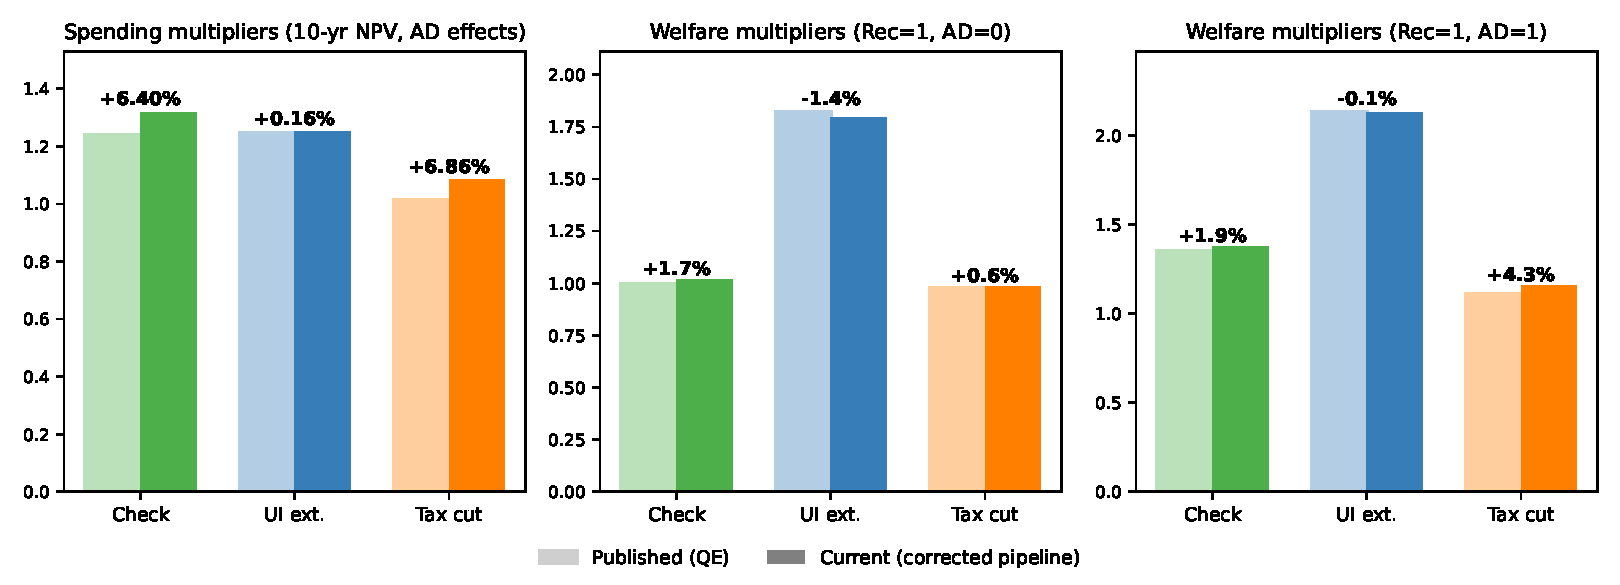
\includegraphics[width=\linewidth]{HAFiscal_update_figs/pe_published_vs_current.pdf}}{}
\caption{PE multipliers, published (QE, hatched) vs.\ the corrected
pipeline (solid), with percent changes. Left: 10-year NPV spending
multipliers (changes $+0.01\%/+0.05\%/+0.07\%$). Center and right: the
\texttt{welfare6} recession rows without and with aggregate-demand
effects (UI $-3.9\%$ and $-1.4\%$; check $+1.6/+2.4\%$; tax cut
$+0.6/+5.2\%$). Seed-to-seed SE from the three-seed whole-cell band:
$\approx$0.02--0.03 on the UI cells, $\le$0.006 elsewhere --- the UI
changes are within noise; the others are small but real. Regenerates
via \texttt{Code/HA-Models/update\_figs.py} from the frozen QE tables
and the certified current battery pickles.}
\label{fig:pecompare}
\end{figure} Exact bit-for-bit reproduction of the
published numbers is preserved separately (the frozen publication
branch/tag; the \texttt{HAFISCAL\_QE\_FIDELITY=1} flag reproduces the
published \emph{construction}, with results within a few percent of
the publication where stochastic machinery differs). Cross-architecture
reproduction and a from-scratch cold start pass on the corrected
pipeline; a timed cold end-to-end run of the complete pipeline
(estimation through policy comparison, no caches) finished in
\textbf{92 minutes} on my Apple-silicon laptop, versus the 4--5 days
the QE-submitted version quotes in its own README.

\section{HANK-SAM results: published vs.\ corrected}
\label{sec:hank}

The published Section-5 figure reported cumulative spending multipliers
whose three series were computed under an \emph{accidental mix} of
monetary regimes (transfers and tax cut under an active Taylor rule; UI
under a fixed real rate), though the caption described a fixed real
rate. The corrected results are computed under each regime separately;
per my 2026-08-10 decision the \textbf{featured arm is the
active Taylor rule} (the realistic description of policy), with the
\textbf{fixed-real arm reported as the robustness companion} (it is
exactly invariant to the one non-identified object in the model, the
household asset level, and it matches the PE model's fixed-$R$
assumption).

\begin{center}\small
\begin{tabular}{@{}lccc@{}}
\toprule
cumulative spending multiplier & transfers (check) & UI extension & tax cut \\
\midrule
\textbf{Published figure} (mixed regimes, all defects) & 0.652 & 1.484 & 0.701 \\
\midrule
\textbf{Corrected, FEATURED: active Taylor} (peak) & \textbf{1.681} & \textbf{1.789} & \textbf{1.503} \\
\quad at one year / three years & 0.87 / 1.53 & 1.23 / 1.68 & 0.56 / 1.36 \\
\textbf{Corrected, companion: fixed real} ($h{=}20$) & 1.181 & 1.387 & 1.347 \\
\quad at one year / three years & 0.81 / 1.09 & 1.21 / 1.34 & 0.54 / 1.21 \\
\midrule
\emph{new metric:} welfare multiplier ($u'$-weighted), Taylor & 1.313 & 2.456 & 1.211 \\
\emph{new metric:} welfare multiplier, fixed real & 1.230 & 2.402 & 1.299 \\
\bottomrule
\end{tabular}
\end{center}

Headline changes relative to the published figure: (i) all multipliers
are substantially larger once the defects are removed (the published
transfers/tax values were doubly depressed --- by the $\Gamma=1$
calibration defect and by the regime mix); (ii) \textbf{UI extensions
remain first} in the featured arm at every horizon and in both metrics;
(iii) the welfare metric --- new to the corrected machinery: Jacobians
of the population $u'(c)$-weighted consumption response, normalized per
unit of policy cost --- shows UI's dominance most starkly (2.46 vs.\
$\approx$1.2--1.3), driven almost entirely by \emph{within}-group
targeting of high-$u'$ households.

A note on horizons: cumulative multipliers converge as the horizon grows
(essentially all delivered dollars are eventually spent), so long-horizon
values compress differences in spending \emph{speed}. Statements about
MPC-driven differences should quote horizons within the figure's
displayed window ($h\le 12$ quarters); at one year the UI multiplier is
$2.2\times$ the tax cut's in either regime.

\section{The regime findings}
\label{sec:regime}

\subsection{On the corrected artifacts, the active Taylor rule
\emph{amplifies}}

In the published-era construction, moving a series to the active Taylor
rule \emph{damped} it (textbook crowding out). On the corrected
artifacts the sign flips: Taylor multipliers exceed fixed-real by
12--42\%. The mechanism is the \textbf{net-creditor interest-income
channel}: households own the entire government bond stock (calibrated to
data, $\approx$31\% of annual GDP), so when the Taylor rule raises rates
into the policy boom, the hikes are income transfers \emph{to}
households, and the income effect dominates intertemporal substitution.
The fingerprint is the monotone regime ordering
$\text{Taylor} > \text{fixed real} > \text{fixed nominal}$
(under a fixed nominal rate, inflation lowers the real rate and cuts
creditor income; those peaks are lowest, 0.80/1.21/0.87).

Two qualifications. First, the Taylor-arm \emph{levels} --- and even
the Taylor arm's \emph{position in the ordering} --- inherit the
model's one non-identified object, the household asset level: both the
interest-income flow and the long-bond revaluation loss scale with the
bond stock. Re-measured on the exact featured artifacts (2026-08-10):
under the full-consistency treatment that feeds the household block's
own aggregate wealth into the bond slot ($\approx$4.1$\times$ the
data-calibrated stock; rejected as a calibration by the closure
appendix), the featured trio $1.68/1.79/1.50$ falls to
$0.84/1.11/0.86$ --- the Taylor arm flips from amplifying to damping
and the regime ordering reverses (fixed nominal highest). At the
data-calibrated 31\%-of-GDP bond stock, the featured numbers and the
ordering above stand. The fixed-real companion is \emph{exactly}
invariant across both treatments (1.1806/1.3871/1.3465 to four
decimals) --- one more reason it is the robustness companion. (An
earlier draft quoted a pre-featuring sensitivity band,
$\rightarrow 2.80/2.73/2.31$, with orderings ``robust across the
band''; that was measured on pre-chains artifacts and is superseded
by this measurement.) Second, any crowding-out prose
keyed to the published figure is backwards on the corrected artifacts.

\subsection{The incidence inversion}

Decomposing the featured transfers experiment instrument-by-instrument
through the education-specific welfare Jacobians shows that under the
active Taylor rule \textbf{the composition of the boom inverts}: the
rate response cools hiring from impact (the job-finding path is negative
throughout), and the positive spending multiplier is carried by the
wealth channel (bond-holders' interest income and the inflation-lifted
wage path). The distributional consequence: dropout households --- the
most unemployment-exposed group, now correctly carrying their calibrated
8.5\% risk after BUG-076 --- are made \emph{worse off} by checks
($-1.46$ in welfare-multiplier units: employment channel $-4.7$, tax
path $-2.1$, against wage $+3.9$ and near-zero bond income) and by tax
cuts ($-0.40$), while \textbf{UI extensions remain strongly positive
for them} ($+3.4$; the direct benefit dominates). Under the realistic
monetary rule, UI is the only one of the three policies whose benefits
reach the unemployment-exposed. The fixed-real companion shows no such
inversion (all groups benefit from all three policies).

\section{The two roles of the tax rate (an investigation, withdrawn as
a correction, kept as a lesson)}
\label{sec:tau}

The HANK-SAM block's households pay $\tau=0.3$ while the PE model has no
taxes; the fiscal ledger's government consumption $G_{ss}\approx 26\%$
of output is computed as a residual and never discussed. I initially
filed this as an inconsistency and executed the alternative at full
depth: a \emph{derived} minimal-government rate ($\tau^{*}=4.07\%$,
funding exactly the modeled UI outlays and debt interest with $G=0$),
shared by both models, with the calibration re-estimated to match. The
experiment refuted its own premise: every multiplier inflated by
$\times 1.33$, and the per-instrument decomposition proved why --- the
tax rate is the model's \textbf{automatic stabilizer}. Of each marginal
unit of output, households' take-home claim scales with $(1-\tau)$; the
$\tau$-slice leaks to a budget that does not recycle it at the margin.
$\tau=0.3$ therefore plays two roles at once, both at roughly realistic
values: the \emph{average} rate financing a realistically-sized
government (whose expenditure $G$ the PE model deliberately abstracts
from), and the \emph{marginal} leakage damping the demand loop (the US
tax-and-transfer system claws back $\approx$25--40\% of marginal income
fluctuations). A flat tax cannot separate the roles, and a
minimal-government rate serves neither realistically. The published
design is a feature; what it lacked was only documentation --- the
sentence this section supplies. (En route this investigation surfaced
and fixed the genuine BUG-076, and produced measured sensitivities kept
as robustness numbers: re-estimating the discount factors under a full
30\% disposable-income convention moves spending multipliers $-25\%$
with every ranking intact; the wedge's effect on the estimated splurge
is $+1.1\%$.)

\section{Why the two models' amplification mechanisms differ}
\label{sec:window}

The PE model's demand amplification is \emph{assumed} (income responds
to aggregate consumption with elasticity 0.3) and is switched on
\textbf{only during the recession} (expected duration $\approx$6
quarters); spending arriving after exit multiplies one-for-one. The
HANK-SAM block's amplification is \emph{derived} from the labor market
and the fiscal ledger, and --- because the solution is a first-order
sequence-space linearization --- it is \textbf{state-independent by
construction}. Long-horizon cross-model comparisons therefore measure
this design difference more than economics: the slow-spending tax cut
is barely above one in PE (1.016: its backloaded spending misses the
recession window) but 1.35--1.50 in HANK (the always-on loop amplifies
the tail), while the front-loaded check inverts the sign (PE 1.239
vs.\ HANK fixed-real 1.181). Each model expresses something the other
cannot: PE, that demand externalities operate in slack conditions;
HANK, a loop derived from structure rather than assumed. The fair
comparison zone is the displayed window ($h\le12$), where both
mechanisms are plausibly active.

\section{Corrections to specific published statements}
\label{sec:errata}

\begin{enumerate}\itemsep2pt
\item The Section-5 figure caption's ``under a fixed real rate rule''
  did not describe two of the three published series (transfers, tax
  cut: active Taylor). The corrected featured figure is labeled
  ``active Taylor rule''; the fixed-real companion is labeled as such.
\item The text's description of the tax-cut financing (``a fiscal
  rule'', singular, implying symmetry) did not describe the published
  computation (BUG-074); the corrected computation makes it true.
\item A sign error in the spending-rule feedback description
  ($\varphi_G$): the code was right, the text's sign wrong.
\item The companion tutorial's claims that anticipation effects are
  absent, and that the fixed-real regime implies larger multipliers via
  avoided crowding out, are both artifacts of the defects (BUG-071/072
  and the regime findings above, respectively).
\item The fiscal ledger's UI booking counts only a 0.5-replacement core
  benefit as government outlay, classing the remaining 0.2 for eligible
  recipients as private income --- economically odd bookkeeping,
  immaterial to results, noted for any careful write-up of the fiscal
  block. $\tau$'s financing of $G$ (Section~\ref{sec:tau}) should be
  stated wherever the fiscal block is described.
\end{enumerate}

\section{Reproduction}
\label{sec:repro}

Every number in this document regenerates from the repository:
\texttt{python Code/HA-Models/step4/run\_jacobians.py} ($\approx$10
min) then \texttt{run\_ge.py} (seconds) produces the featured pickle;
the regime cross-table and welfare metrics assemble from the emitted
diagnostics. \texttt{HAFISCAL\_QE\_FIDELITY=1} reproduces the published
construction bit-for-bit through the frozen original scripts. Escape
flags exist for every correction individually (registry:
\texttt{Code/HA-Models/docs/ENV\_FLAGS.md}). The corrected panels below
regenerate via \texttt{Code/HA-Models/update\_figs.py} from the GE
stage's regime-pure diagnostics; the published figure is the frozen
reference. All three panels share the paper's displayed window
($h\le 12$).

\begin{figure}[h!]
\centering
\IfFileExists{images/Cumulative_multipliers_withHank.pdf}{%
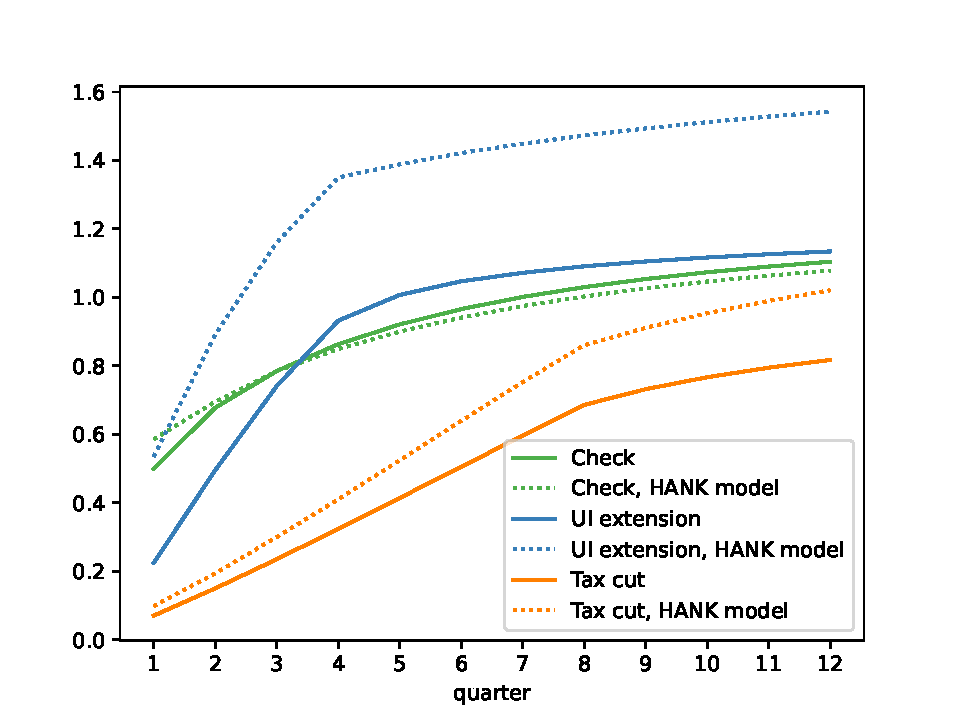
\includegraphics[width=.62\linewidth]{images/Cumulative_multipliers_withHank.pdf}\\
{\small (a) The \emph{published} figure (frozen reference): the
accidental regime mix (transfers/tax under active Taylor, UI under
fixed real), all defects included.}\\[6pt]}{}
\IfFileExists{HAFiscal_update_figs/withHank_taylor.pdf}{%
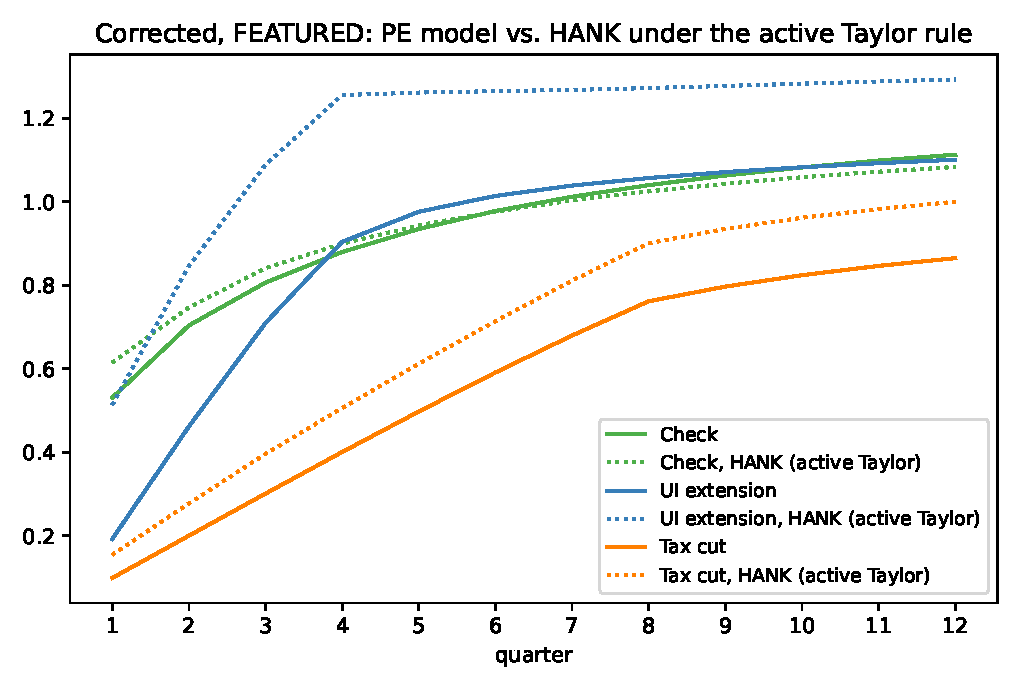
\includegraphics[width=.62\linewidth]{HAFiscal_update_figs/withHank_taylor.pdf}\\
{\small (b) \textbf{Corrected, FEATURED: active Taylor rule.} As in
the published figure, PE model solid, HANK dotted, same colors. The PE
lines are the \emph{corrected-pipeline} PE results ($h{=}12$:
1.07/1.06/0.82; long-run limits 1.2391/1.2487/1.0167, within 0.1\% of
the published table). Corrected HANK under the realistic
monetary rule, $h{=}12$: 1.53 / 1.68 / 1.36 --- above PE throughout:
the wealth-channel amplification of Section~\ref{sec:regime}, whose
levels carry the asset-sensitivity band.}\\[6pt]}{}
\IfFileExists{HAFiscal_update_figs/withHank_fixed_real.pdf}{%
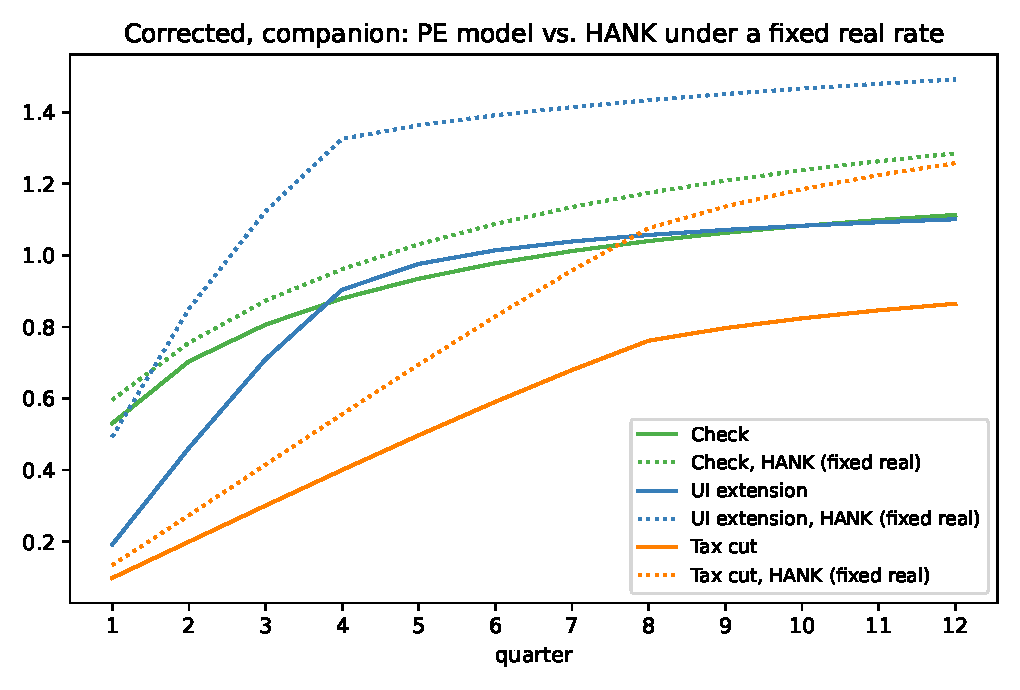
\includegraphics[width=.62\linewidth]{HAFiscal_update_figs/withHank_fixed_real.pdf}\\
{\small (c) \textbf{Corrected, companion: fixed real rate.} The
level-invariant arm, monetary assumptions matched to PE (fixed $R$).
HANK $h{=}12$: 1.09 / 1.34 / 1.21 --- close to the PE lines for the
check, above for UI and (later horizons) the tax cut.}}{}
\caption{Cumulative spending multipliers, PE (solid) vs.\ HANK-SAM
(dotted): the published figure (frozen) and the two corrected arms.
UI extensions lead within the displayed window in every corrected
arm and both models.}
\end{figure}

\end{document}
